\section{Application to vacuum spectra}
\label{sec:results_vacuum}

Now we move to present the application of the strategy presented in the previous
section to the parametrisation of the ZLP spectra taken in vacuum.
%
Applying our model to this case has a two-fold motivation.
%
First of all, we aim to demonstrate that our model is flexible enough to effectively reproduce the
input EELS measurements for a range of variations of the operation parameters of the microscope.
%
Second, it will allow us to provide a calibration prediction for the case of the in-sample measurements.
%
Such calibration is necessary since, as explained in Sect.~\ref{sec:training}, some of the model
hyper-parameters are determined by the comparison of the intensity derivatives
between spectra taken in vacuum and those in sample.

In Table~\ref{table:vacuumdata} we collect the main properties of the EELS spectra acquired in vacuum to train the neural
    network model.  For each set of spectra, we indicate the exposure time $t_{\rm exp}$, the beam energy
    $E_b$, the number of spectra $N_{\rm sp}$ corresponding to these operation conditions, the number $N_{\rm dat}$ of
    bins in each spectrum, the range in electron energy loss $\Delta E$,
    and the average full width at half maximum (FWHM)
    evaluated over the $N_{\rm sp}$ spectra with the corresponding variance.
    %
    The data sets were recorded with a Titan TEM equipped with a Skottky field emitter.
    %
    Since we are interested in the low-loss region, $\Delta E_{\rm max}$ does not need
    to be too large, and in any case the large $|\Delta E|$ behaviour of the model is fixed
    by the constraint implemented by means of Eq.~(\ref{eq:chi2modified}).
    %
    The energy resolution of these spectra, quantified by the value of the FWHM, ranges
    from 3 eV to 25 eV depending on the specific operation conditions of the microscope.
    %
    A total of 81920 independent measurements will be thus used for the ZLP model
    training on the vacuum spectra.
    %
    As we show below, one of the advantages of our model is that it can extrapolate the ZLP predictions
    for other operation conditions of the microscope beyond those used for the training.

%%%%%%%%%%%%%%%%%%%%%%%%%%%%%%%%%%%%%%%%%%%%%%%%%%%%%%%%%%%%%%%%%%%%%%%%%%%%%%%%%%%%%%%%%%%%%
%%%%%%%%%%%%%%%%%%%%%%%%%%%%%%%%%%%%%%%%%%%%%%%%%%%%%%%%%%%%%%%%%%%%%%%%%%%%%%%%%%%%%%%%%%%%%
\begin{table}[t]
  \begin{center}
            \renewcommand{\arraystretch}{1.50}
  \begin{tabular}{@{}ccccccccc}
\br
Set & $t_{\rm exp}$ {(}ms{)} & $E_{\rm b}$ {(}keV{)} & $N_{\rm sp}$ & $N_{\rm dat}$ & $\Delta E_{\rm min}$~(eV)  & $\Delta E_{\rm max}$~(eV)  & FWHM~(eV)  \\ 
\mr
1        & 100                 & 200                  & 15          & 2048               & -0.96              & 8.51     & $0.025\pm$         \\
2        & 100                 & 60                   & 7           & 2048               & -0.54              & 5.59    & $ 0.022\pm$         \\
3        & 10                  & 200                  & 12          & 2048               & -0.18              & 2.97      & $0.003\pm$         \\
4        & 10                  & 60                   & 6           & 2048               & -0.40              & 4.78       & $0.017\pm$         \\ 
\br
  \end{tabular}
    \end{center}
  \caption{\small Summary of the main properties of the EELS spectra acquired in vacuum to train the neural
    network model.  For each set of spectra, we indicate the exposure time $t_{\rm exp}$, the beam energy
    $E_b$, the number of spectra $N_{\rm sp}$ corresponding to these operation conditions, the number $N_{\rm dat}$ of
    bins in each spectrum, the range in electron energy loss $\Delta E$,
    and the average FWHM evaluated over the $N_{\rm sp}$ spectra with the corresponding variance.
  }
   \label{table:vacuumdata}
\end{table}
%%%%%%%%%%%%%%%%%%%%%%%%%%%%%%%%%%%%%%%%%%%%%%%%%%%%%%%%%%%%%%%%%%%%%%%%%%%%%%%%%%%%%%%%%%%%%%%%%5
%%%%%%%%%%%%%%%%%%%%%%%%%%%%%%%%%%%%%%%%%%%%%%%%%%%%%%%%%%%%%%%%%%%%%%%%%%%%%%%%%%%%%%%%%%%%%

Following the strategy presented in Sect.~\ref{sec:methodology}, first of all we combine the $N_{\rm sp}$ spectra
corresponding to each of the four sets of operation conditions and determine the statistical uncertainty
associated to each energy loss bin by means of Eq.~(\ref{eq:sigmaiexp}).
%
We use this information to generate a sample of $N_{\rm rep}=500$ Monte Carlo replicas of the input data listed
in Table~\ref{table:vacuumdata} and train an individual neural network model to each of these replicas.
%
The end result of the procedure is a set of model replicas, $I_{\rm ZLP}^{\rm (mod)(k)}(\Delta E, E_{b},t_{\rm exp})$,
which can be used to provide a prediction for the intensity of the ZLP
for arbitrary values of $\Delta E$,  $E_{b}$, and $t_{\rm exp}$.
%
This sample provides a representation of the probability density in the space of $I_{\rm ZLP}$ models, from which
statistical estimators such as averages, variances, and correlations can be evaluated by means of
the standard MC expressions, namely
\be
\la I_{\rm ZLP}^{\rm (mod)}(\Delta E, E_{b},t_{\rm exp}) \ra = \frac{1}{N_{\rm rep}}\sum_{k=1}^{N_{\rm rep}}
I_{\rm ZLP}^{\rm (mod)(k)}(\Delta E, E_{b},t_{\rm exp}) \, ,
\ee
\be
\sigma_{I_{\rm ZLP}}^{\rm (mod)}(\Delta E, E_{b},t_{\rm exp})  = \lp \frac{1}{N_{\rm rep}-1} \sum_{k=1}^{N_{\rm rep}}
\lp  I_{\rm ZLP}^{\rm (mod)(k)}  - \la I_{\rm ZLP}^{\rm (mod)}  \ra   \rp \rp^{1/2} \, ,
\ee
\be
\rho \lp \{z_1\},\{z_2\}\rp = \frac{ \la I_{\rm ZLP}^{\rm (mod)}( \{z_1\} ) I_{\rm ZLP}^{\rm (mod)}( \{z_2\} ) \ra
- \la I_{\rm ZLP}^{\rm (mod)}( \{z_1\} )\ra \la I_{\rm ZLP}^{\rm (mod)}( \{z_2\} ) \ra}{\sigma_{I_{\rm ZLP}}^{\rm (mod)}( \{z_1\} )\sigma_{I_{\rm ZLP}}^{\rm (mod)}( \{z_2\} )}
\ee
where as in the previous section $\{z_l\}$ denotes a possible set of input variables for the model.
We now discuss some of features of this ZLP vacuum model.

\paragraph{Fit quality.}
%
To begin with we would like to quantify the overall fit quality of the model and demonstrate that it is flexible enough
to describe all the available input datasets.
%
In Table~\ref{table:chi2summary} we indicate the values of the final $\chi^2$ per data point,
    Eq.~(\ref{eq:chi2_final}), as well as the average values of the error Eq.~(\ref{eq:chi2})
    over the training and validation subsets, for each of the four sets of spectra listed in
    Table~\ref{table:vacuumdata} as well as for the total dataset.
    %
    We recall that for a satisfactory training one expects $\chi^2 \simeq 1$
    and $\la E_{\rm tr}\ra \simeq \la E_{\rm val}\ra \simeq 2 $~\cite{Forte:2002fg}.
    %
    From the results of this table we can see that ....

%%%%%%%%%%%%%%%%%%%%%%%%%%%%%%%%%%%%%%%%%%%%%%%%%%%%%%%%%%%%%%%%%%%%%%%%%%%%%%%%%%%%%%%%%%%%%
%%%%%%%%%%%%%%%%%%%%%%%%%%%%%%%%%%%%%%%%%%%%%%%%%%%%%%%%%%%%%%%%%%%%%%%%%%%%%%%%%%%%%%%%%%%%%
\begin{table}[t]
  \begin{center}
            \renewcommand{\arraystretch}{1.35}
  \begin{tabular}{@{}cccc}
\br
Set & $\chi^2$  &  $\la E_{\rm tr}\ra$   &  $\la E_{\rm val}\ra$ \\
\mr
1        &                 &                  &    \\
2        &                  &                   &      \\
3        &                   &                   &     \\
4        &                   &                    &      \\
\mr
Total    &                     &                      &      \\
\br
  \end{tabular}
    \end{center}
  \caption{\small The values of the final $\chi^2$ per data point,
    Eq.~(\ref{eq:chi2_final}), as well as the average values of the error Eq.~(\ref{eq:chi2})
    over the training and validation subsets, for each of the four sets of spectra listed in
    Table~\ref{table:vacuumdata} as well as for the total dataset.
  }
   \label{table:chi2summary}
\end{table}
%%%%%%%%%%%%%%%%%%%%%%%%%%%%%%%%%%%%%%%%%%%%%%%%%%%%%%%%%%%%%%%%%%%%%%%%%%%%%%%%%%%%%%%%%%%%%%%%%5
%%%%%%%%%%%%%%%%%%%%%%%%%%%%%%%%%%%%%%%%%%%%%%%%%%%%%%%%%%%%%%%%%%%%%%%%%%%%%%%%%%%%%%%%%%%%%

\subsubsection{Energy loss}
\label{sec:eloss}

The full energy range of the vacuum recorded peaks covers an interval varying from -1 to +9 eV. In order to test the flexibility of the network with respect to extrapolation on the energy interval, a window was applied to restrict the training loss values to [-0.2, 0.05] eV. Prediction inputs for exposure time and beam energy were kept the same as training values; the energy loss was extrapolated between [-0.5, 0.5] eV. After training the neural network on each MC replica, the best network parametrization was stored and used later for the prediction, such that from the ensemble of predictions the central values and uncertainties could be calculated. The results for the four different vacuum peaks can be observed in Fig.~\ref{fig:extrapoleloss} below. 

\begin{figure}[H]
    \centering
    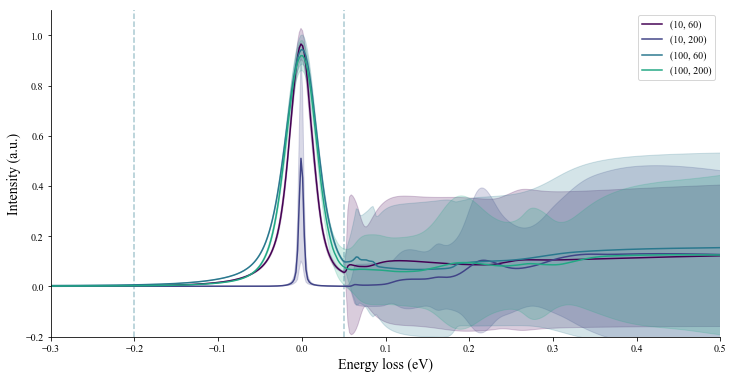
\includegraphics[width=120mm]{plots/extrapolate_energyloss.png}
    \caption{Energy loss extrapolation on vacuum peaks under four different recording settings (exposure time, beam energy). The data within the energy region [-.2, 0.05] eV is known to the network by training. Extrapolation predictions are shown outside this region, marked by the dashed lines.}
    \label{fig:extrapoleloss}
\end{figure}

The goodness of our prediction can be quantified by means of $\chi^2$. So one can separate the parameter space (in Texp and Ebeam for example) into "training" and "prediction" regions, and use one to predict the other. If our error estimate is good, we should find chi2/ndat $\simeq$ 1 also for the predicted datasets


\subsubsection{Beam energy}
\label{sec:ebeam}
The training data contained only two recorded beam energies of 60 and 200 keV. Interpolation and extrapolation predictions have been retrieved on a continuous set of beam energies between 0 and 300 keV. In Fig.~\ref{fig:extrapolbeam} one can observe the mean predicted intensity and mean prediction error, where the average is taken over the energy loss range. The dashed lines indicate the beam energies for which we have data: correspondingly, the errors in these points are small, as the model can make an accurate prediction. The more the beam energy deviates from the known values, the bigger the uncertainties in the predictions become. 

\begin{figure}[H]
    \centering
    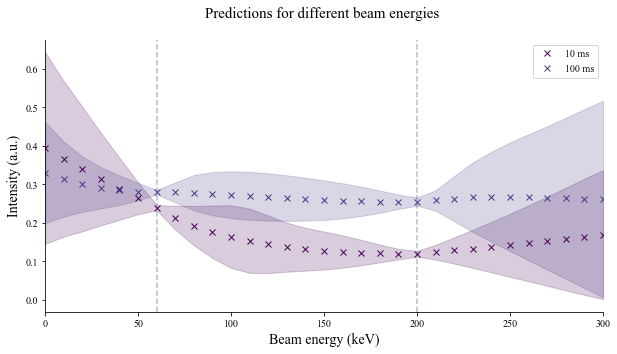
\includegraphics[width=120mm]{plots/Extrapolate_beamenergy.png}
    \caption{Predictions on a continuous set of beam energies, while inputs for energy loss and exposure time are the same as for the training data. The dashed lines indicate the beam energies that are known to the network by training.}
    \label{fig:extrapolbeam}
\end{figure}

\subsubsection{Exposure time}
\label{sec:texp}
The network was trained on data with exposure times of $10$ and $100$ ms, so interpolation and extrapolation is possible. Similar to the predictions for varying beam energy, also for exposure time the uncertainties grow bigger as the value deviates more from the training inputs.

\begin{figure}[H]
    \centering
    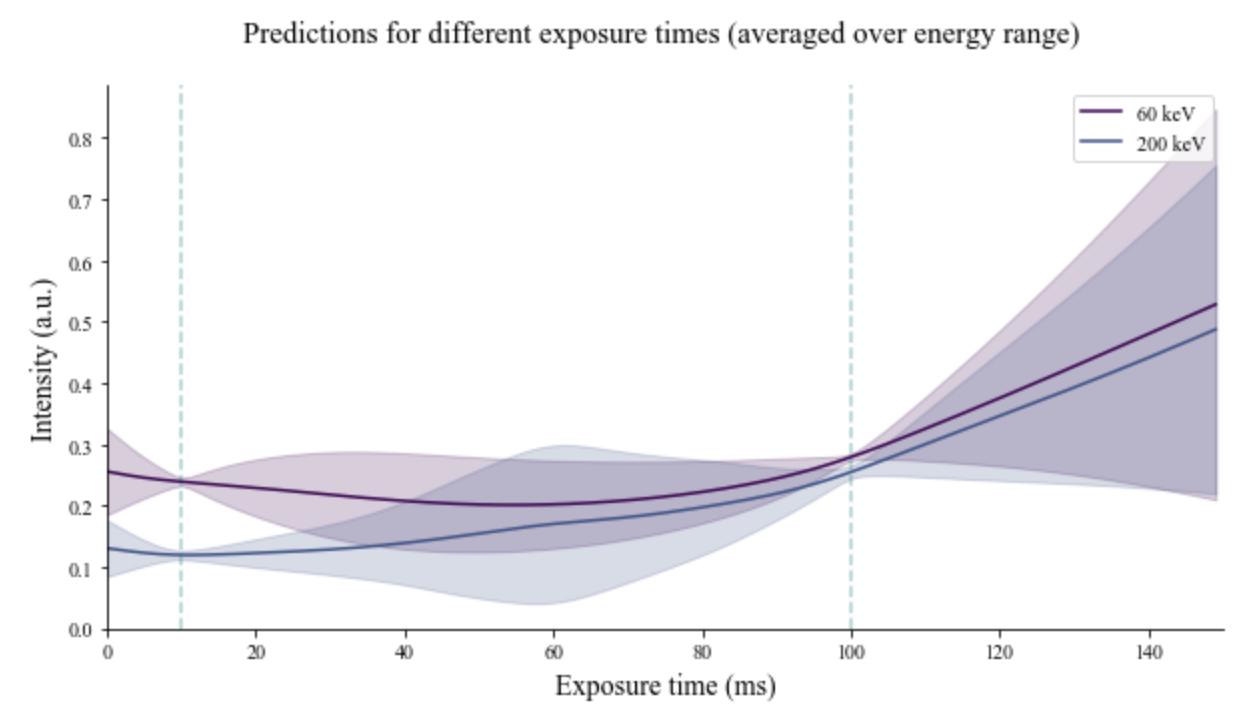
\includegraphics[width=120mm]{plots/Extrapolate_exposuretime.png}
    \caption{Predictions on a continuous set of exposure time, while inputs for energy loss and beam energy are the same as for the training data. The dashed lines indicate the exposure times known to the network by training.}
    \label{fig:extrapolbeam}
\end{figure}
